\clearpage
\section{Event Reconstruction}
\label{sec:EventReconstruction}

\subsection{P\cancel{0}D and Tracker Reconstruction Algorithms}

The \p0d Reconstruction is a stand alone reconstruction algorithm 
that uses hits measured in the scintillator bars and combines them 
into tracks and showers. 
These \p0d-only track objects are then passed on to the matching 
algorithm described later in this section. 
A detailed description of the \p0d Reconstruction algorithm 
can be found in T2K-TN-072 \cite{tn72}. \\

The Tracker Reconstruction algorithm 
similarly reconstructs tracks passing through the Tracker region of ND280. 
The ND280 Tracker is consists of three TPCs and two Fine Grain Detectors (FGD) 
in between the TPCs. 
In General the Tracker 
%For the Tracker tracks used in this CC inclusive analysis, 
the resonstruction algorithm uses TPC tracks 
in the YZ projection (the non-drift direction) 
as a seed to reconstruct tracks from hits in the FGDs. 
To reconstruce TPC tracks in the XZ projection 
(i.e. the drift direction), 
a T0 is extracted from either the matched FGD hits, the cathode 
or one of the surrounding subdetector 
such as the \p0d, barrel ECal or \p0d ECal. 
Greater detail on the construction of, and the algorithms responsible 
for reconstructing tracks passing through, 
the Tracker can also be found in T2K-TN-072 \cite{tn72}.

%\subsection{Algorithm for Matching Together P\cancel{0}D and Tracker Tracks}
\subsection{Tracker-to-\p0d Matching Algorithm}
\label{sec:MatchingAlgorithm}

The tracks match algorithm is base on the reconstruction output objects of 
both \p0d and Tracker reconstruction packages.
The algorithm pair a \p0d track that ends in the downstream part of teh \p0d with a Tracker track that start in the upstream part of TPC1 
(i.e. most upstream part of the Tracker).
%
%We take the resultant tracks of the \p0d and tracker reconstruction packages and match them together using a `homebrew' reconstruction algorithm. This homebrew matching algorithm pairs \p0d and tracker tracks together in a one-to-one fashion and is the last step of reconstruction before selection cuts are applied. 
In this section we describe the matching algorithm in more details.

\subsubsection{Description of Algorithm}

The matching procedure can be divided into two stages - in 
the first stage the outputs of \p0d and Tracker reconstruction are 
scanned, while in the second stage a list of pair-candidates 
is generated for later purpose. \\

At the first stage the algorithm scan for candidate \p0d and Tracker tracks. 
These tracks need to pass quality and position checks, 
in addition to the time window requirement of $\pm100$ ns from each other. 
This time cut is set to be able to reject tracks from different bunches 
on one hand, and on the other hand to take into account possible uncertainties 
or difference between sub-detectors calibrated time stamps.\\

The \p0d track tests at this stage are:
\begin{itemize}
\item 
The track passes through the downstream part of the \p0d. \\
i.e. Last node Z position \(>\) -1016 mm.
\item 
The track should be a 3D track. \\
To determine this a check of the track position variance is done, 
each coordinate $X_{var}$, $Y_{var}$ and $Z_{var}$ should be 
smaller then the large value of 
%\(<\) 
$10^8$ mm.
\end{itemize}

The Tracker track tests at this stage are:
\begin{itemize}
\item 
The track start position is at the upstream part of the Tracker.\\
i.e. The first node Z position \(<\) -750 mm.
\item 
The track should have more than 18 nodes.
\end{itemize}

In the second stage the algorithm identifies 
all possible pair-candidates. 
At first the algorithm creates a list of pair-candidates from 
%This is done by pairing 
all combinations of candidate \p0d and Tracker tracks 
(outputs of the first stage).
For each candidate pair the algorithm collects information for later usage 
(like - Bunch number, Tracker track change, \p0d track start position) 
and calculates, in addition, the momentum of the pair-candidate at the start 
position of the \p0d track 
(more details about this in Sec. \ref{sec:EnergyCorrection}) 
as will as the two matching parameters 
$\Delta R$, $sin\Delta\theta$. \\
%matching parameters 
%properties 
%of each pair-candidate.
%, which are used later in the matching procedure. 
Figure \ref{fig::dRsinTcalc} illustrates the above matching parameters 
$\Delta R$ and $sin\Delta\theta$. 
Where $\Delta R$ is the radial distance (in the XY plane) 
between the most downstream \p0d track node 
and the Tracker track linear backwards projection to the same Z position 
as that last \p0d track node, 
and $\Delta\theta$ (which we apply a $sin$ on) is the angle 
%difference 
between the \p0d track last node direction and the Tracker track direction 
(see Figure \ref{fig::dRsinTcalc} right side).

At the last part of this stage the algorithm sorts out pair-candidates 
which did not satisfy the matching cut conditions of $\Delta R < 0.76\ mm$ 
and $sin\Delta\theta < 0.86$ 
(more details on how the matching values have be obtained are laid out 
in Sec \ref{MatchCutOpt}).
\\

\begin{figure}
\centering
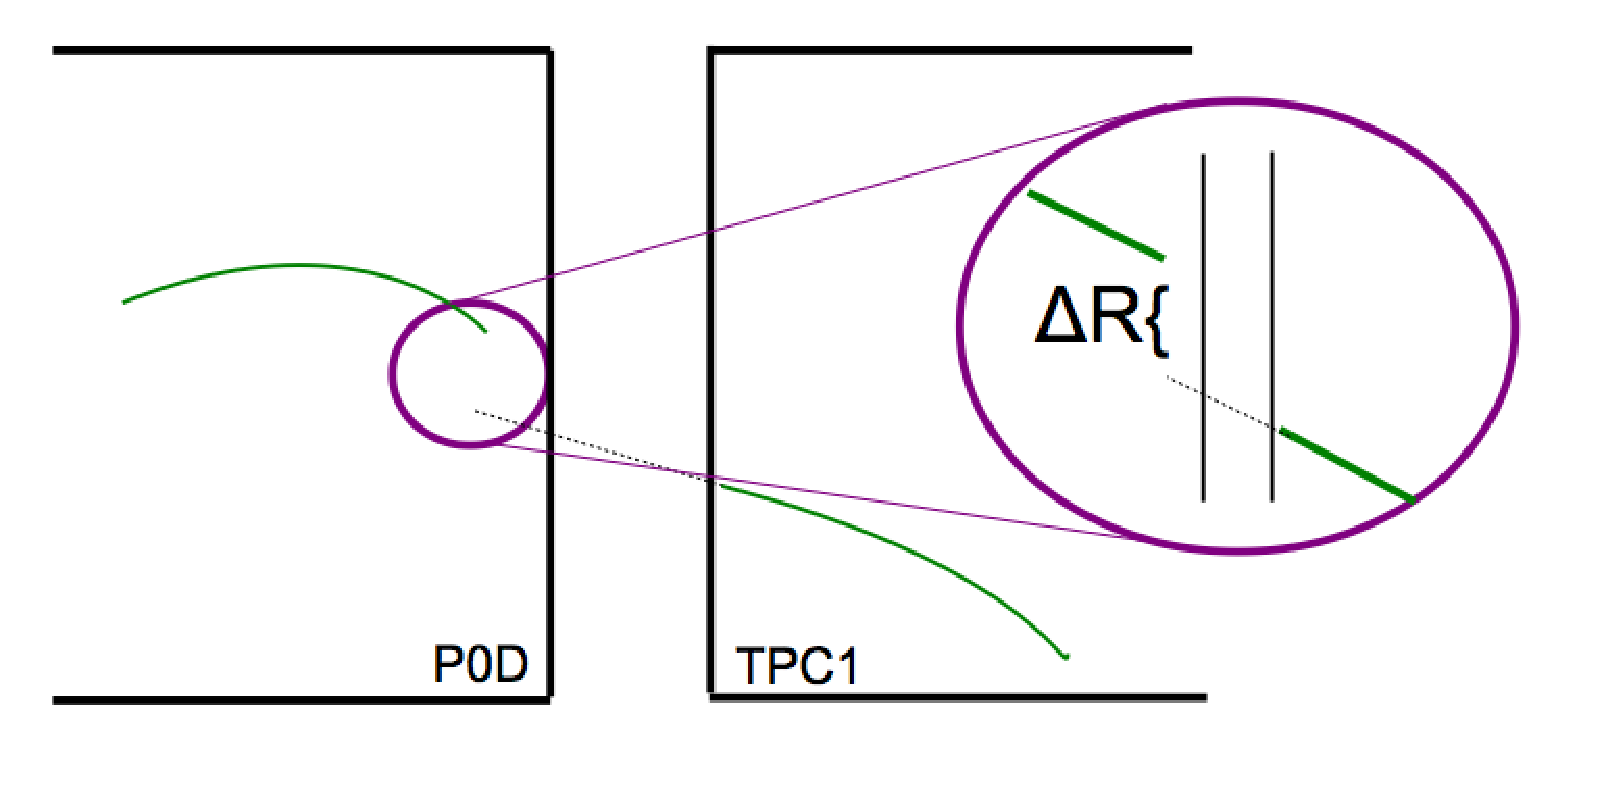
\includegraphics[width=3in]{Figures/drCalc.eps}
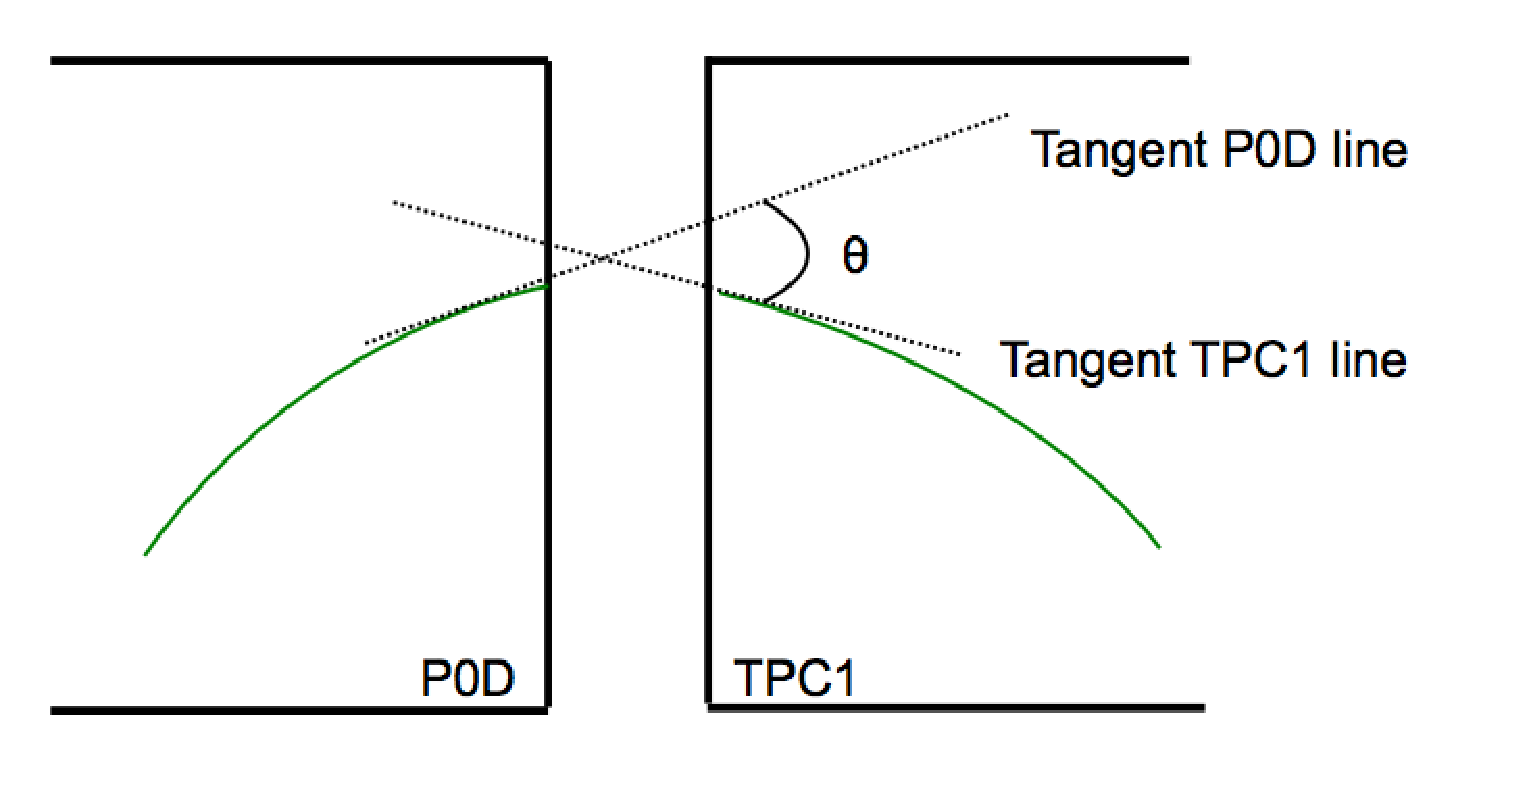
\includegraphics[width=3in]{Figures/sindThetaCalc.eps}
\caption{
Diagrams 
%which illustrate 
of the \(\Delta R\) and \(\sin \Delta \theta\) matching parameters. 
Both parameters are extracted 
%calculated 
with the use of position and direction information 
of the \p0d track last node 
and Tracker track first node.
The \(\Delta R\) (\(\sin \Delta \theta\)) parameter 
is illustrated on the left (right).
}
\label{fig::dRsinTcalc}
\end{figure}

%In the last stage the algorithm identifies the highest momentum negative 
%track in a bunch and tags it as the muon candidate of that event.

In addition the algorithm makes sure that 
any \p0d or Tracker track candidate (output of the first stage) 
is used only once, i.e. appears only in a pair-candidate which has the 
smallest $\Delta R$ value.

%(the way this is achieved is by sorting 
%all candidate pairs by their $\Delta R$ value, 
%then selecting pair-candidates with the smallest $\Delta R$, 
%where any other pair-candidate pairs that includes 
%one of the selected (\p0d or Tracker) tracks are ignored).

%Once track candidates have been selected in each event, they are passed to the matching algorithm. For every combination of one \p0d track and one Tracker track, we calculate the three matching parameters $\sin\Delta\theta$, $\Delta R$ and $\Delta T$. Figure \ref{fig::dRsinTcalc} shows how $\sin\Delta\theta$ and $\Delta R$ are calculated for each combination. The Tracker track is linearly projected backwards to the same Z position as the most downstream node of the \p0d track. The radial distance between the most downstream \p0d node and the projected position of the Tracker track is $\Delta R$. The angle between the tangent line at the end of the \p0d track and the tangent at the beginning of the Tracker track is $\Delta\theta$. We take take the sine of this angle and use $\sin\Delta\theta$ as another matching parameter. Finally, $\Delta T$ is simply the difference in time stamp between the \p0d and Tracker tracks.

%A list is generated with every possible combination of one \p0d track 
%and one Tracker track. Any combination with a $\Delta T$ \(>\) 100 ns 
%is immediately removed. The timing cut is small enough to reject any 
%combinations of tracks from two different beam bunches 
%but large enough to account for uncertainties in sub-detector timing 
%calibration. 
%Then the combination with the smallest $\Delta R$ value is selected 
%as a `matched track candidate'. 
%Any other combinations using one of the track pieces in this `matched track 
%candidate' are removed from the list of possible combinations. 
%Then the next available combination with the smallest $\Delta R$ 
%is selected as the second `matched track candidate' in the event. 
%This process is repeated until the list of combinations is empty. 
%Finally, any `matched track candidates' 
%with a $\Delta R$ \(>\) 86 mm or a $\sin\Delta\theta$ \(>\) 0.76 
%is rejected as a poor match. 
%The remaning combinations are all considered to be succesfully matched tracks. 

\subsubsection{Opimization of Matching Parameters}
\label{MatchCutOpt}

To determine the cut values used 
%at the end of 
by the matching algorithm described above, 
we used the different MC samples.
A figure of merit was calculated for a range of cut values of $\Delta R$ and $\sin\Delta\theta$ and the pair of values that yields the highest figure of merit is used for the matching algorithm. We chose the figure of merit $ F = \frac{S}{\delta S}$, where S is the number of signal events and $\delta S$ is the error, to minimize the error on the signal. 

We begin with the same matching algorithm described above upto the 
final $\Delta R$ and $\sin\Delta\theta$ cuts, which are not applied. 

The signal (S) is defined as any matched track where both 
the reconstructed \p0d and Tracker track pieces originated 
from the same true primary trajectory 
(a primary trajectory is a true trajectory leaving the interaction vertex). 
The background (B) is the remainder of the matched tracks that do not satisfy 
the signal requirement. 
The errors $\delta S$ and $\delta B$ are the poissonian error on S and B 
respectively. For each pair of cut values (X, Y), 
we count up the total matched tracks that satisfy 
both $\Delta R$ \(<\) X and $\sin\Delta\theta$ \(<\) Y. 
Each matched track is then classified as either signal or background, 
which yields S and B. Finally we calculate the figure of merit which, 
using Poisson error, reduces to ($ F = \frac{S^2+2 B^2}{M^2}$ ). 
Figures \ref{fig:FOMRun2water} and \ref{fig:FOMRun3air} 
shows the figure of merit as a function of 
the cut values for Watre-in (Run 2) and Water-out (Run3) MC samples 
respectively. 
We find local maximas at (76 mm, 0.88) and (78 mm, 0.90) 
for Water0in (Run2) and Water-out (Run 3) respectively. 
For simplicity 
%and backward compatibility, 
we use the values 
%from Run 2 
of 
%$\Delta R \le$ 86 mm and $\sin\Delta\theta \le$ 0.76 
$\Delta R \le$ 76 mm and $\sin\Delta\theta \le$ 0.88 
for the different samples and run periods.

\begin{figure}
\centering
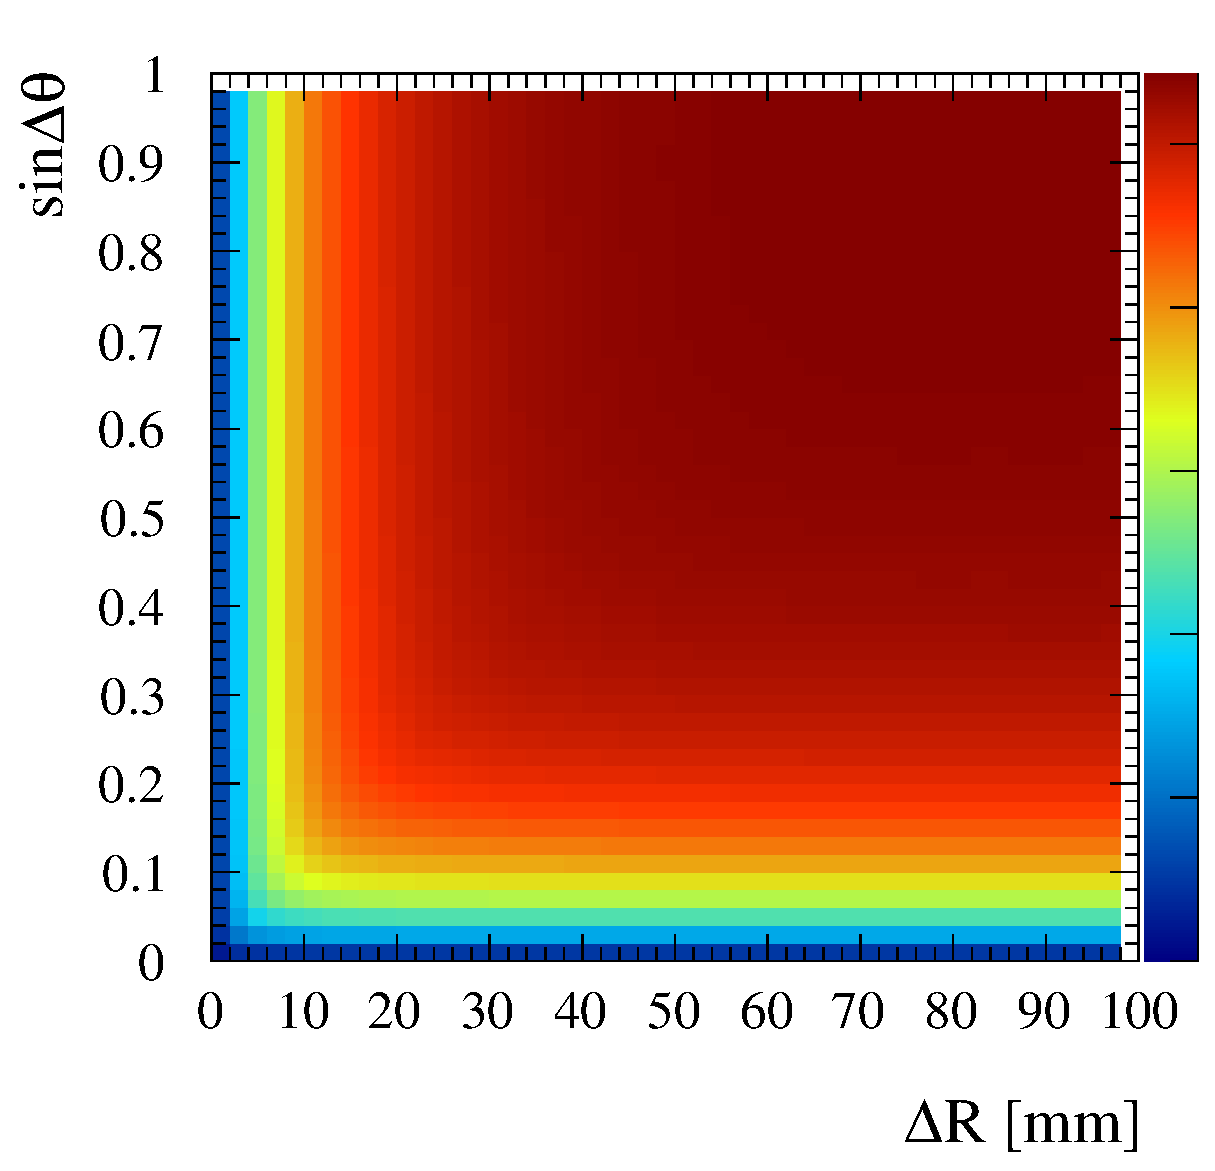
\includegraphics[width=3in]{Figures/optCut-5E-Run2water-caseA-sinTdR-unzoomZ.eps}
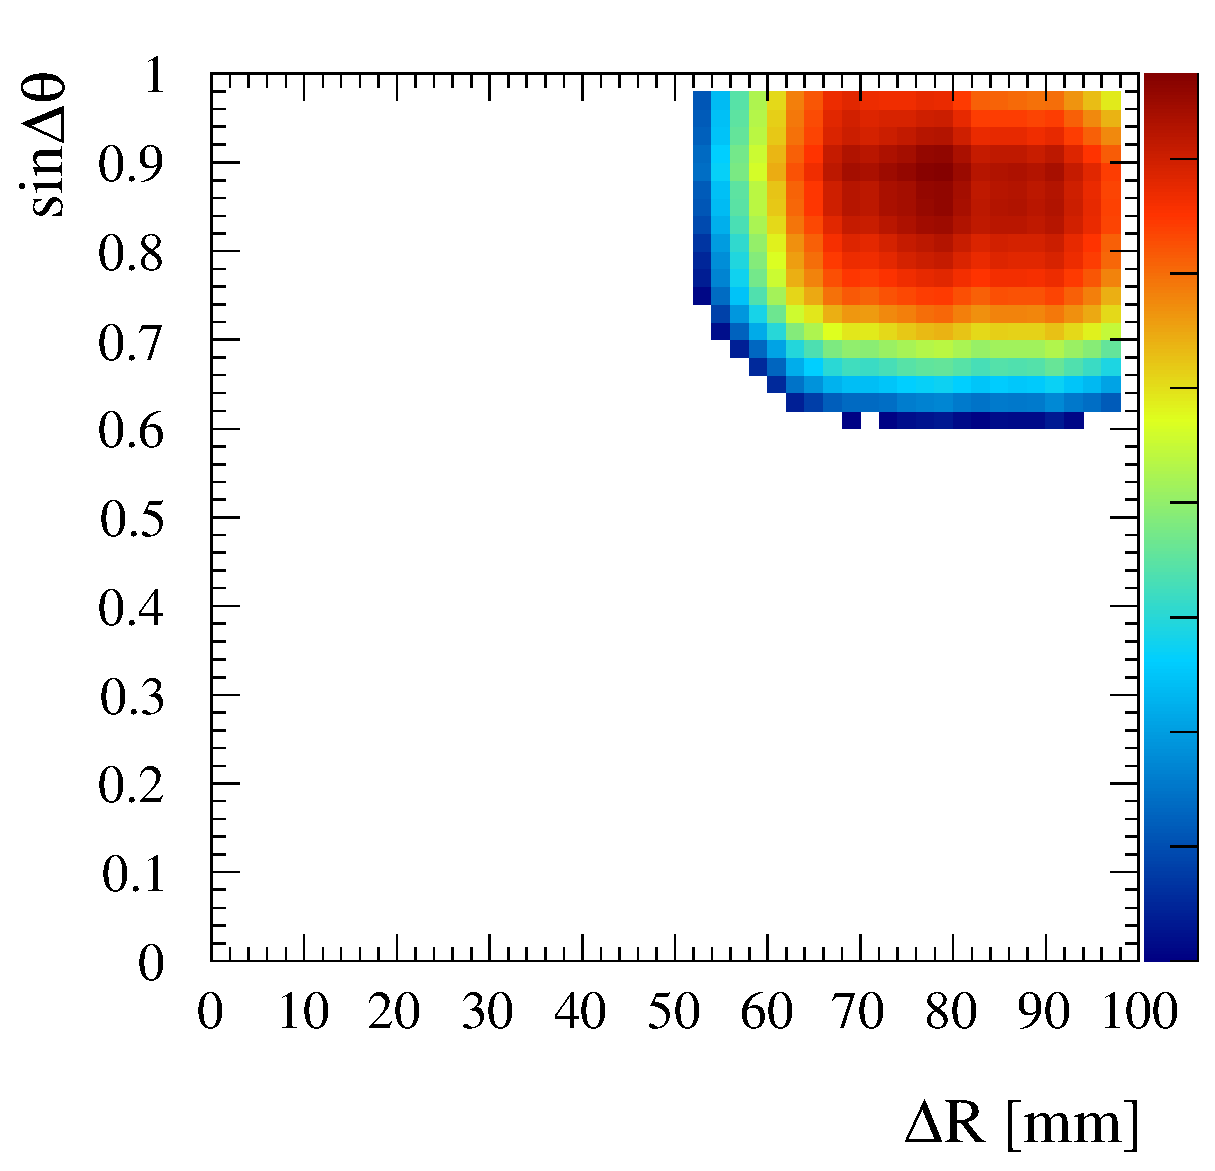
\includegraphics[width=3in]{Figures/optCut-5E-Run2water-caseA-sinTdR-zoomZ.eps}
\caption{The Figure of Merit as a function of $\Delta R$ 
and $\sin\Delta\theta$ for candidate matched tracks from Water-in MC samples 
(Run 2). 
the absolute figure of merit does not vary much in the region of interest. 
The Z-axis zoomed version (right) shows the location of 
the local maxima (76 mm, 0.88).} 
\label{fig:FOMRun2water}
\end{figure}

\begin{figure}
\centering
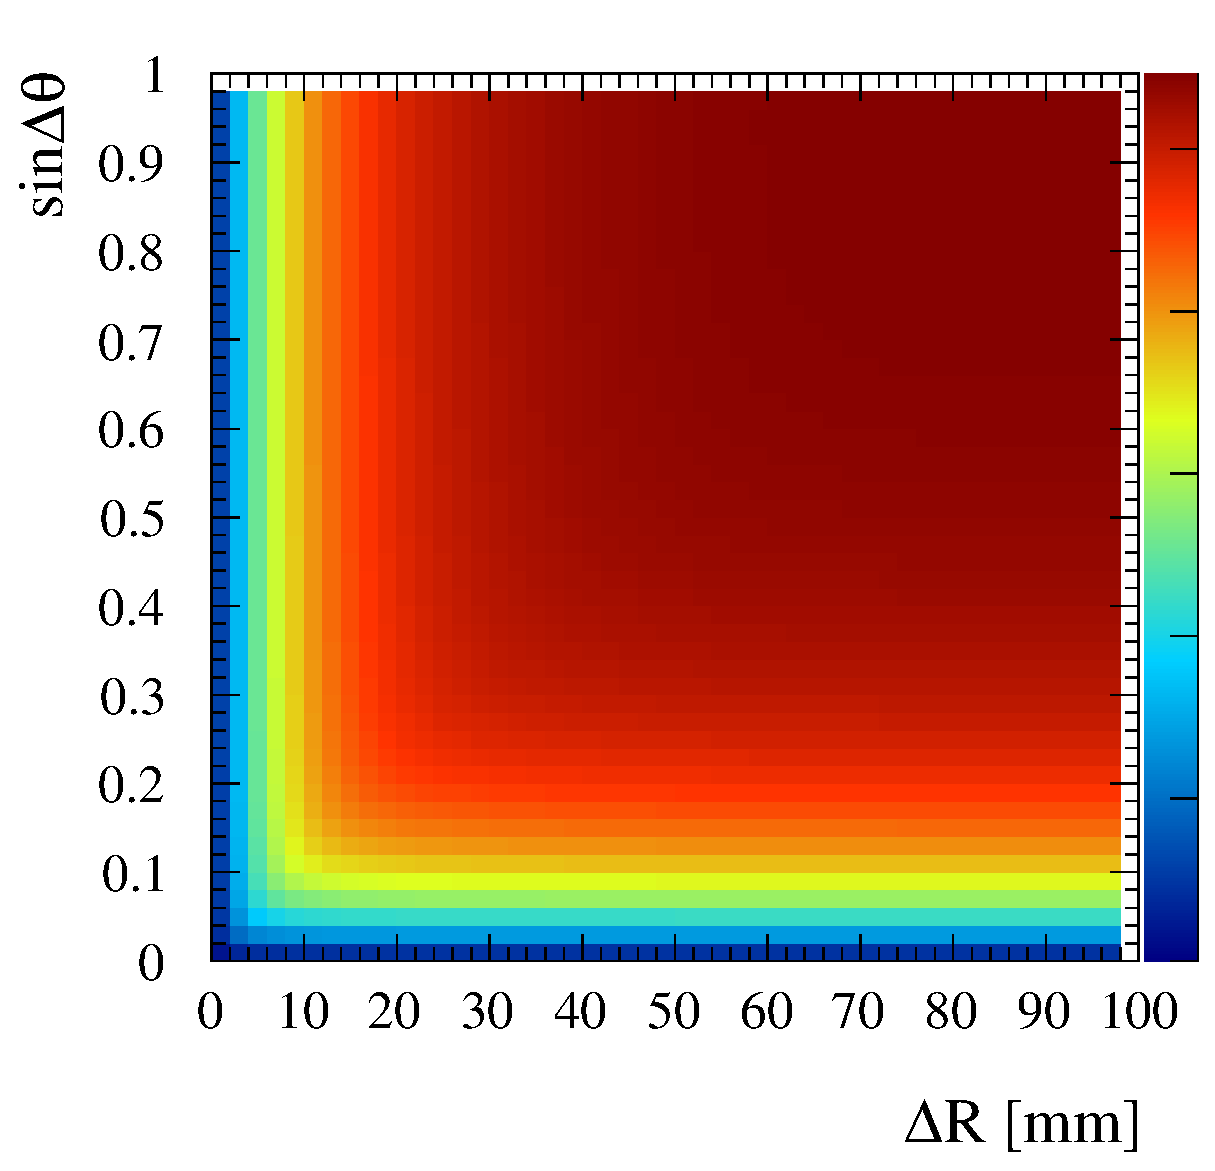
\includegraphics[width=3in]{Figures/optCut-5E-Run3air-caseA-sinTdR-unzoomZ.eps}
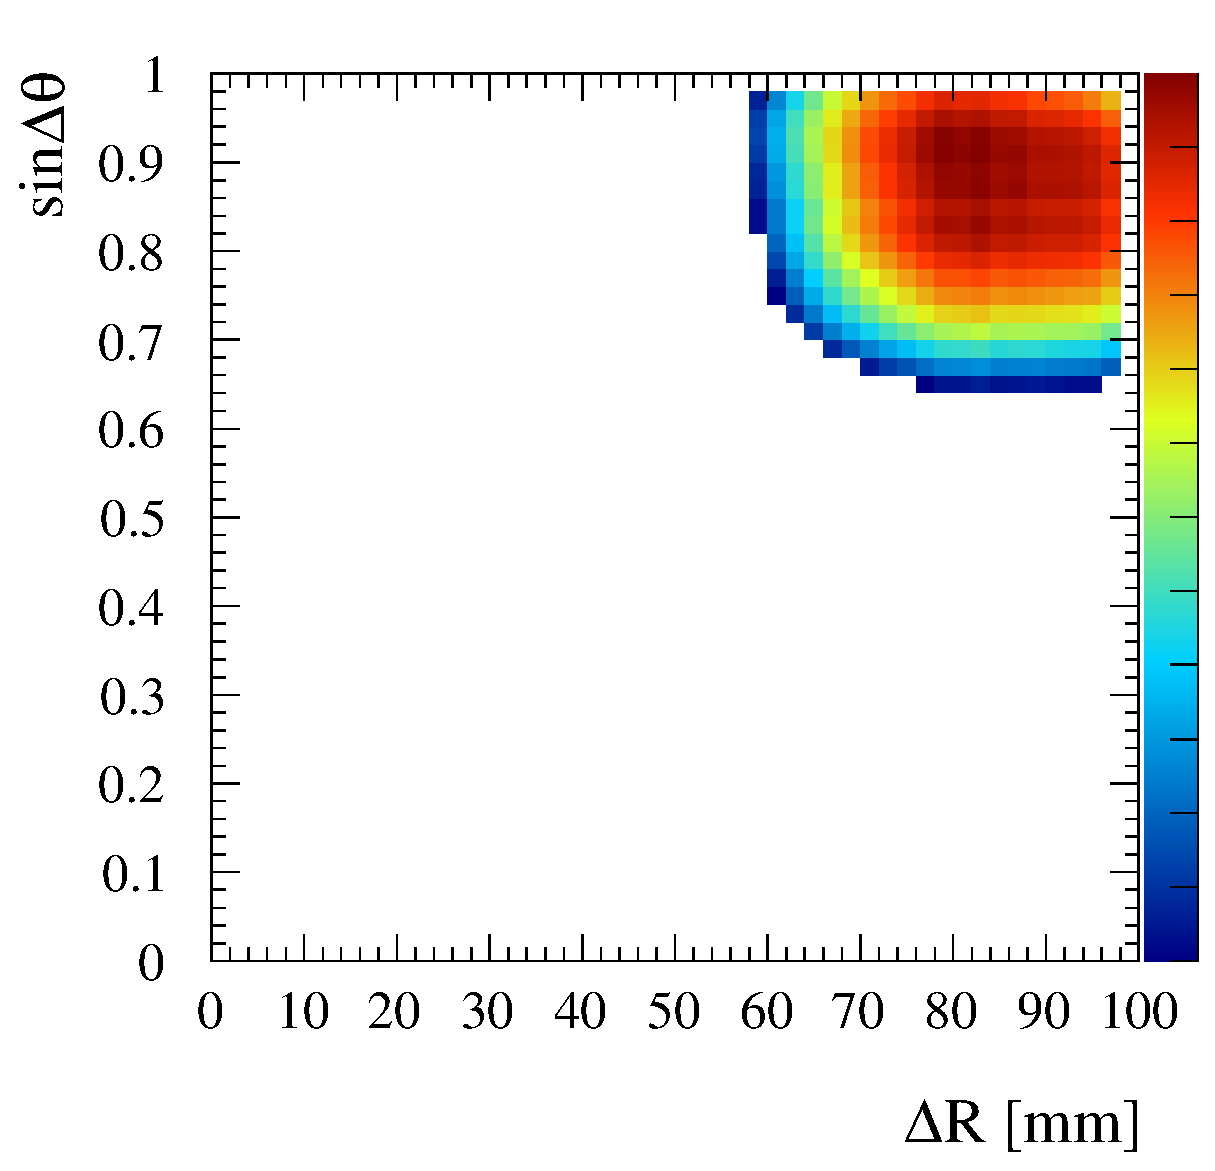
\includegraphics[width=3in]{Figures/optCut-5E-Run3air-caseA-sinTdR-zoomZ.eps}
\caption{The Figure of Merit as a function of $\Delta R$ 
and $\sin\Delta\theta$ for candidate matched tracks from Water-out MC samples 
(Run 3). 
The Z-axis unzoomed version (left) demonstrates that 
the absolute figure of merit does not vary much in the region of interest. 
The Z-axis zoomed version (right) shows the location of 
the local maxima (78 mm, 0.90).} 
\label{fig:FOMRun3air}
\end{figure}

We also note that the local maxima is not 'sharp'. A variation in 
the cut values does not drastically alter the overall figure of merit. 
Also, as the cuts are placed in generally flat regions 
of the $\Delta R$ and $\sin\Delta\theta$ distributions, 
cut value variations do not yield large changes in total tracks reconstructed. 

Finally, as Data and MC distributions of the matching parameters 
show excellent agreement near the cut values, 
variations will not affect the Data/MC ratios. 
These points are demonstrated in Figures \ref{fig:dRsindTWaterIn} and 
\ref{fig:dRsindTWaterOut}, which shows the overall 
pre-cut $\Delta R$ and $\sin\Delta\theta$ distributions of matched track 
candidates in Data and MC. 
Systematic effects resulting from this matching algorithm 
are evaluated later in the efficiency systematic section.

\begin{figure}
\centering
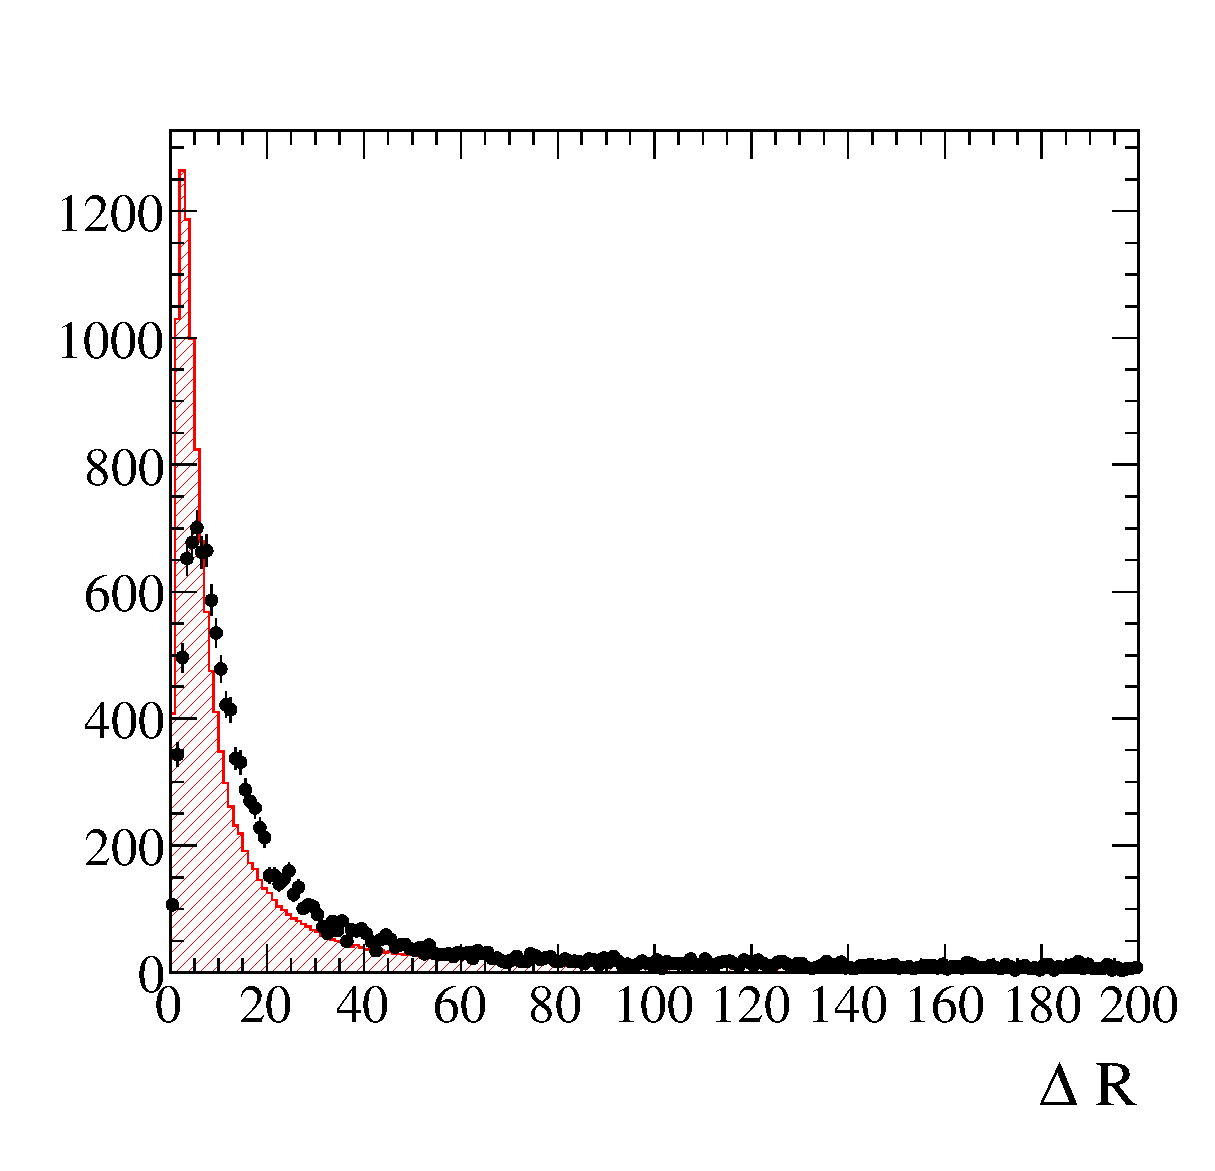
\includegraphics[width=3in]{Figures/optCut-5FE-Run2water-dR-DoMC.eps}
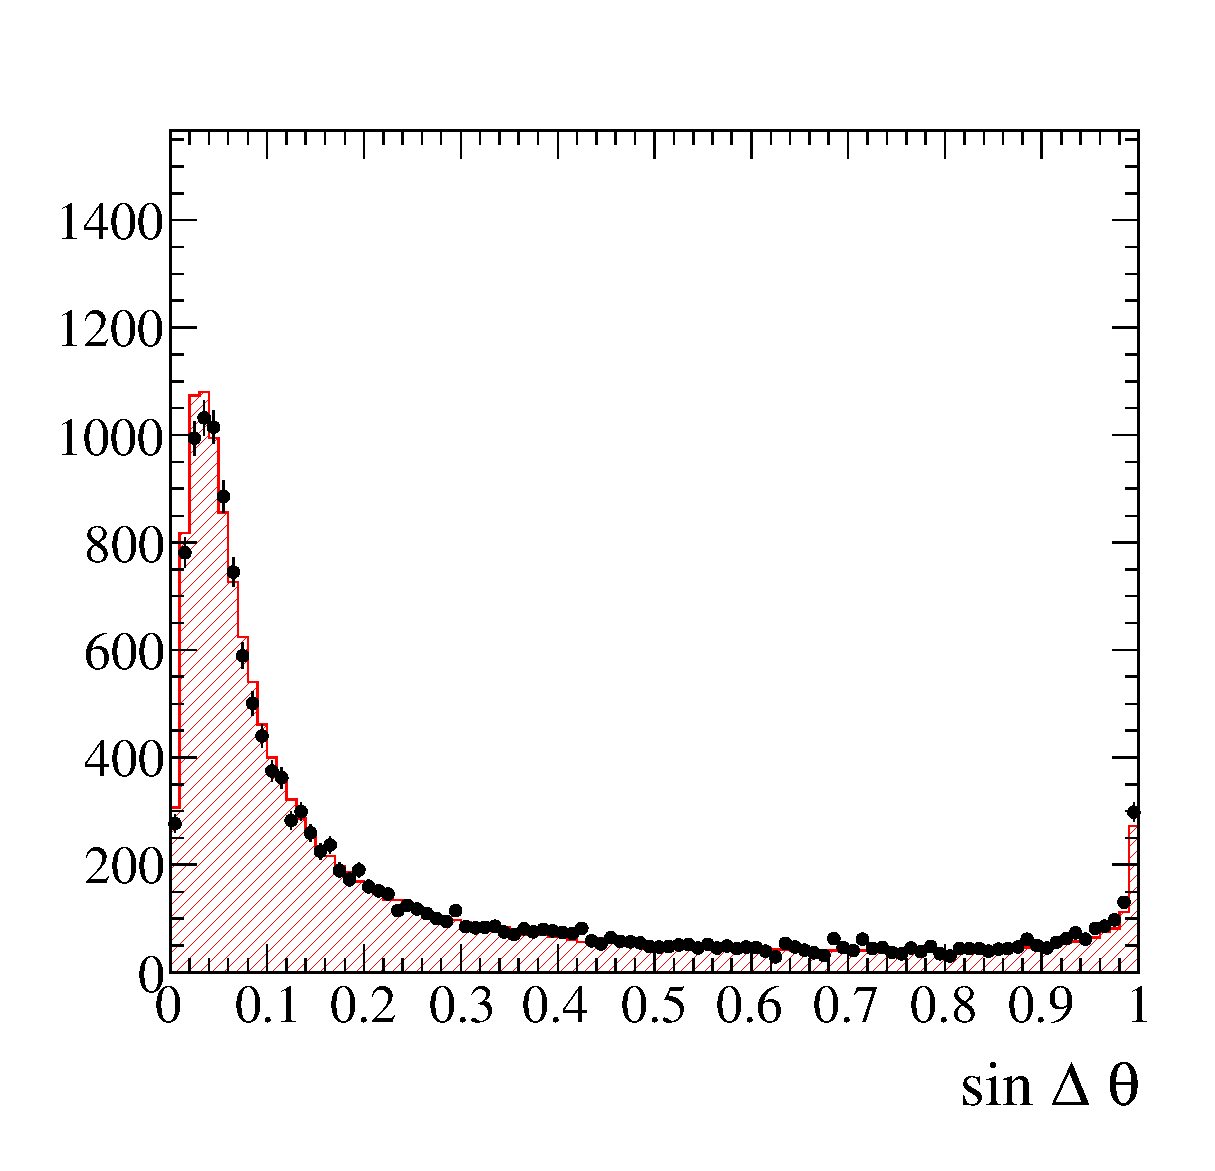
\includegraphics[width=3in]{Figures/optCut-5FE-Run2water-sinT-DoMC.eps}
\caption{The $\Delta R$ (left) and $\sin\Delta\theta$ (right) 
distributions for Water-in samples (Run 2). 
The Data (black) is overlayed on MC (red). 
To be able to compare the MC to the Data, which includes sand interactions 
a cut on the start of the tracks was apply, i.e. Z $> -3183$ mm, 
$|X|$ and $|Y| < 1000$ mm.}
\label{fig:dRsindTWaterIn}
\end{figure}

\begin{figure}
\centering
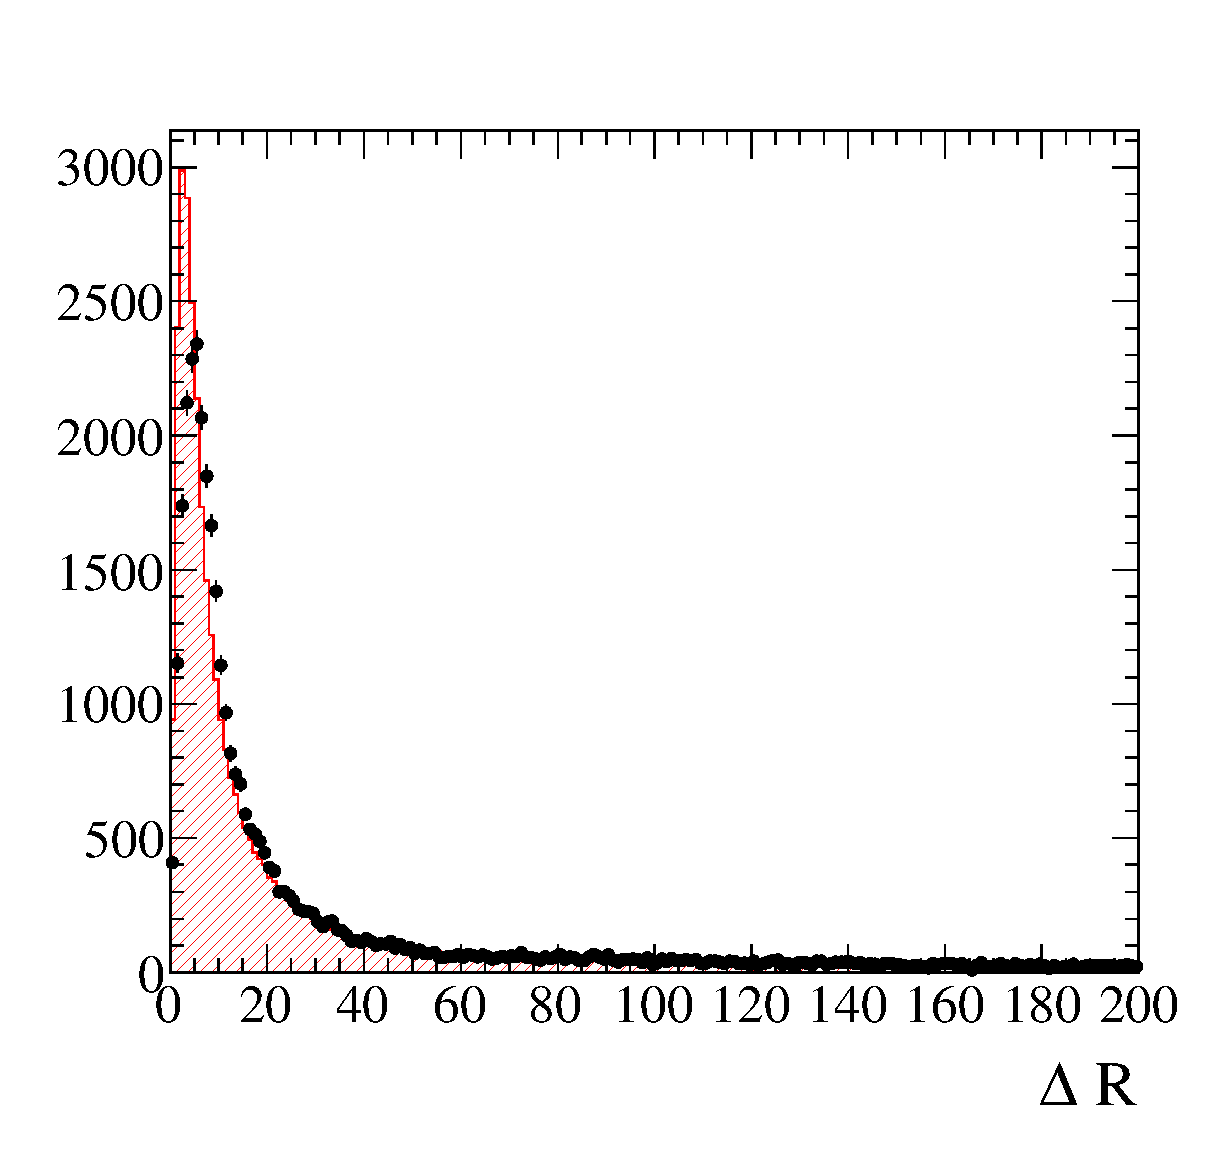
\includegraphics[width=3in]{Figures/optCut-5FE-Run3air-dR-DoMC.eps}
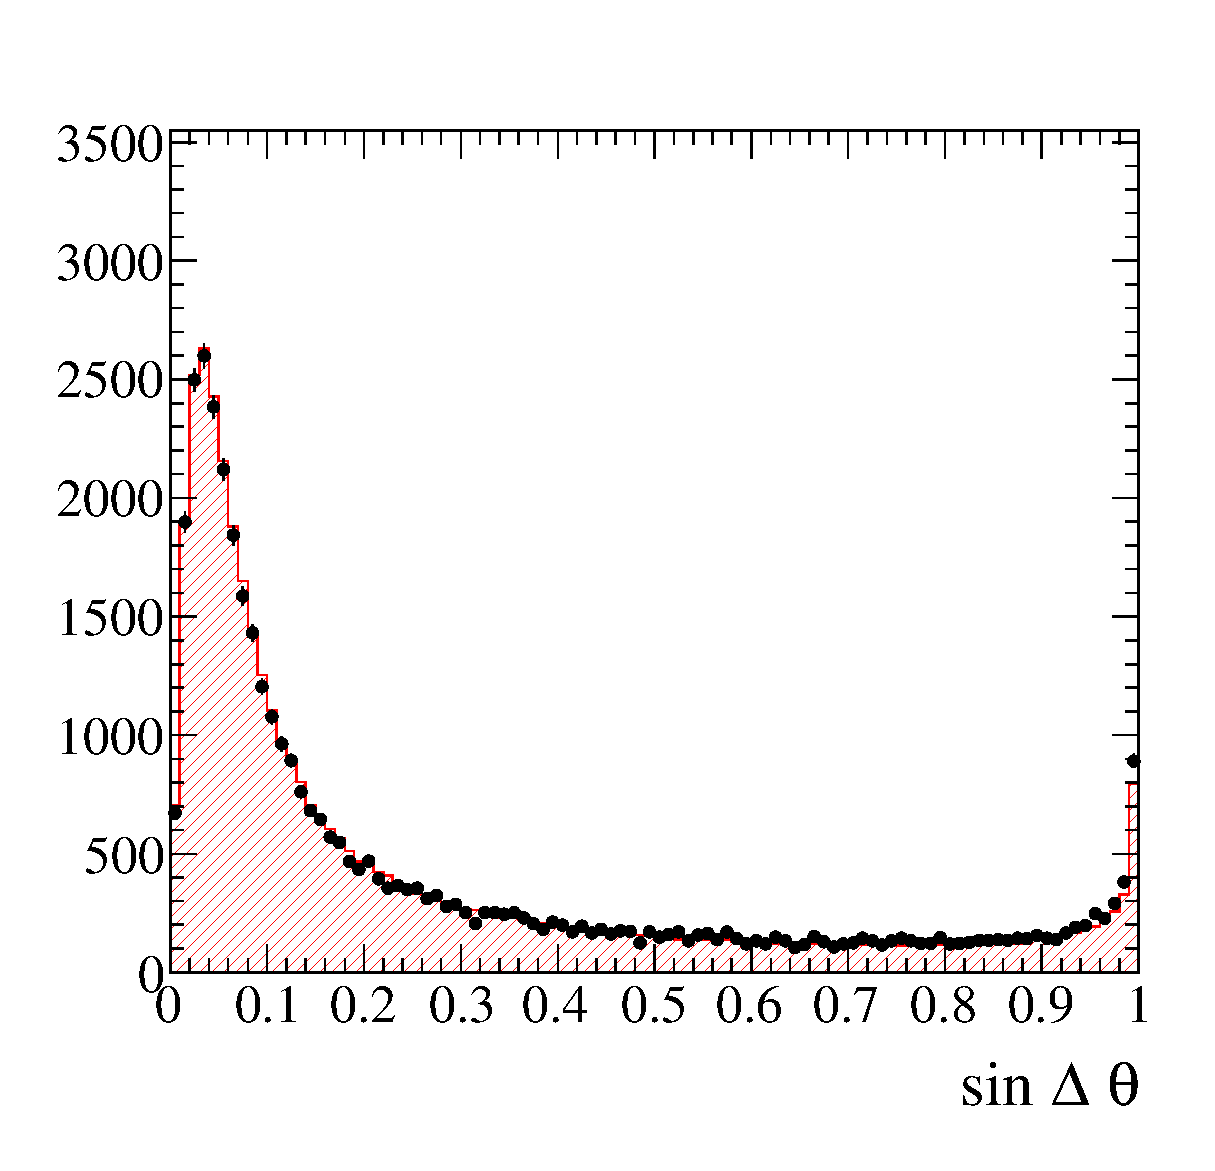
\includegraphics[width=3in]{Figures/optCut-5FE-Run3air-sinT-DoMC.eps}
\caption{The $\Delta R$ (left) and $\sin\Delta\theta$ (right) 
distributions for Water-out samples (Run 3). 
The Data (black) is overlayed on MC (red). 
To be able to compare the MC to the Data, which includes sand interactions 
a cut on the start of the tracks was apply, i.e. Z $> -3183$ mm, 
$|X|$ and $|Y| < 1000$ mm.}
\label{fig:dRsindTWaterOut}
\end{figure}

\subsection{Energy correction in the \p0d}
\label{sec:EnergyCorrection}

Our analysis selects CC inclusive events by tagging the muon candidate. To reconstruct the momentum of the muon candidate, we use the measured TPC1 momentum in conjunction with the length of the track in the \p0d. Using range tables for a muon and our known material density in the \p0d we can calculate the momentum of the muon at the vertex by adding in the expected energy lost. In order for the energy loss correction to be fast, we chose not to use 
$\frac{dE}{dx}$ tables and incrementally adjust the energy. The \p0d energy loss was calculated using range data for the various super\p0dules.
Range is defined as $R(E')=\int^{E'}_0 \left(\frac{dE}{dx}\right)^{-1}\,dE$, where
$\frac{dE}{dx}$ is the weighted average over all materials, and is calculated for each super\p0dule.  
This gave us a table of range vs energy/momentum for every part of the \p0d and 
essentially allowed us to perform the integration once as opposed to for every track.
To obtain the energy lost in the \p0d, we simply take the TPC1 momentum, find its 
corresponding range, add the length of the track in next super\p0dule, and find
the corresponding momentum (see Figure \ref{fig:energyCorr}).  We repeat this as 
necessary depending on whether the track traversed through more than one super\p0dule.

Figure \ref{fig:correctedECompare} shows the residuals of the calculated muon momentum. For comparison, we also provide the muon momentum residual as measured by another independent reconstruction package called `Global Reconstruction'. The residual distribution from the outlined method above shows no bias and a marked improvement over the momentum calculation of global reconstruction. We use only the above method to calculate muon momentum in our analysis.

\begin{figure}
\centering
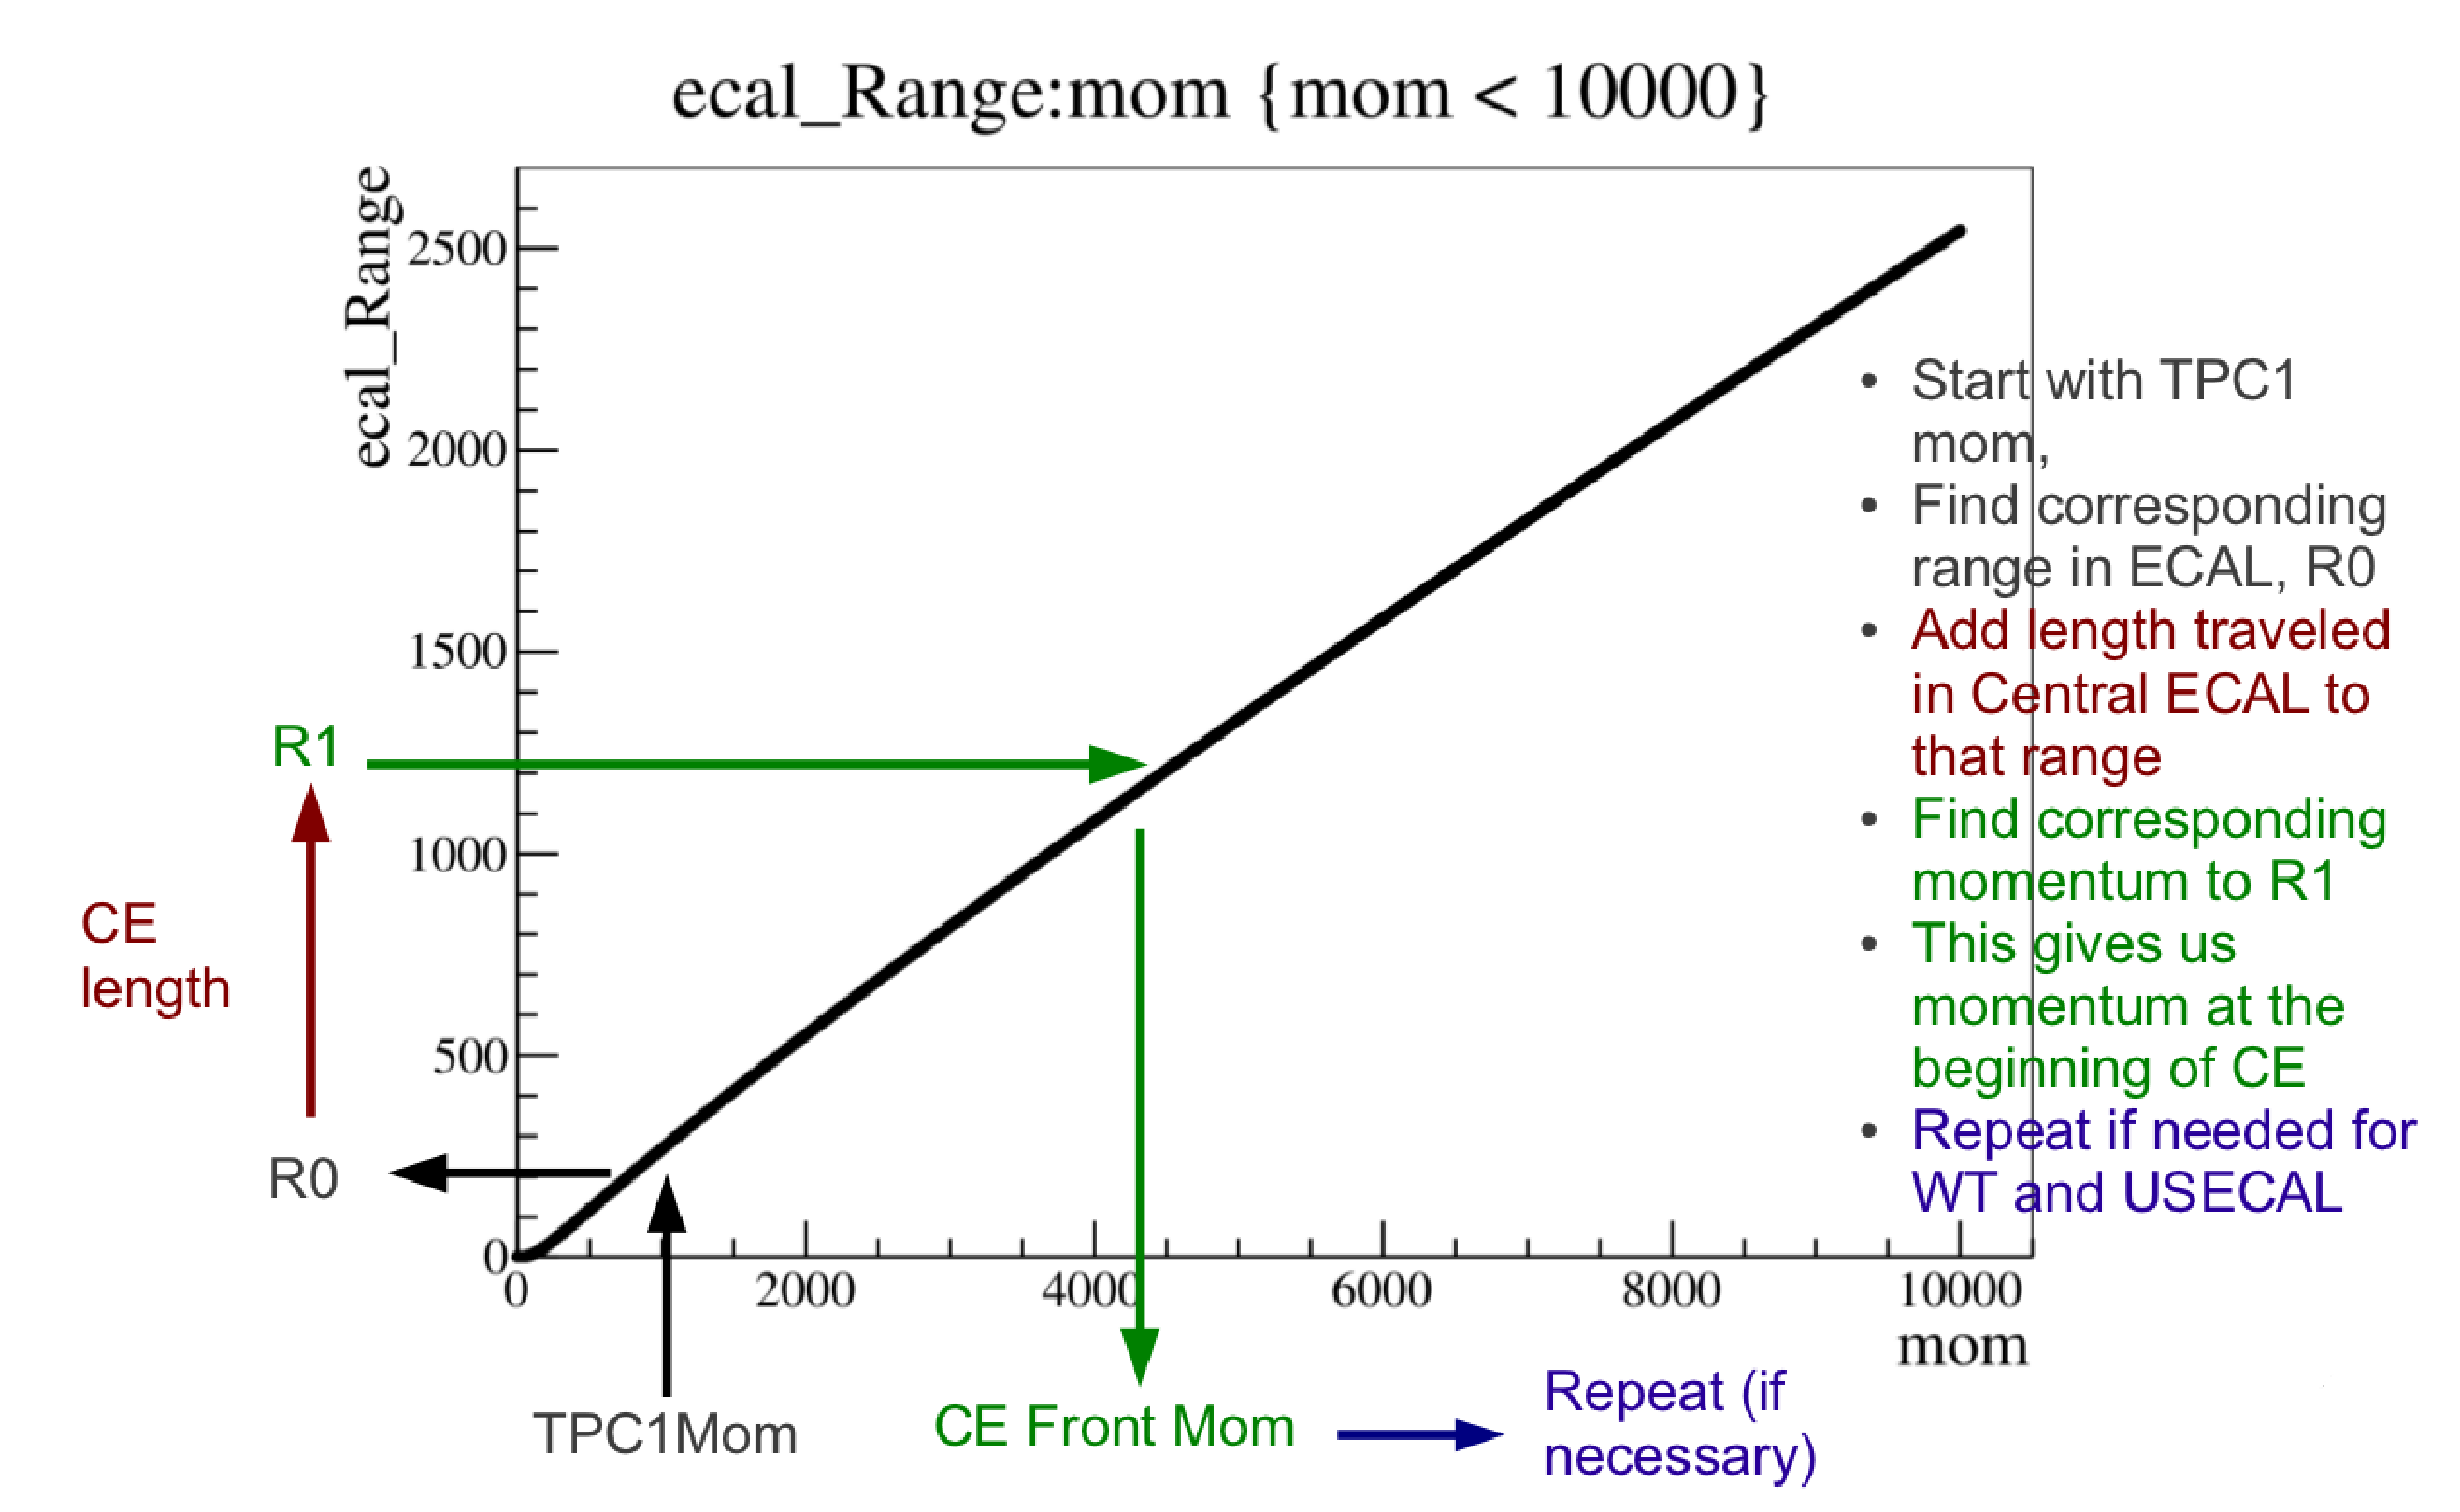
\includegraphics[width=5.5in]{Figures/eLossCalc1.eps}
\caption{Calculation of \p0d momentum correction.} 
\label{fig:energyCorr}
\end{figure}

\begin{figure}
\centering
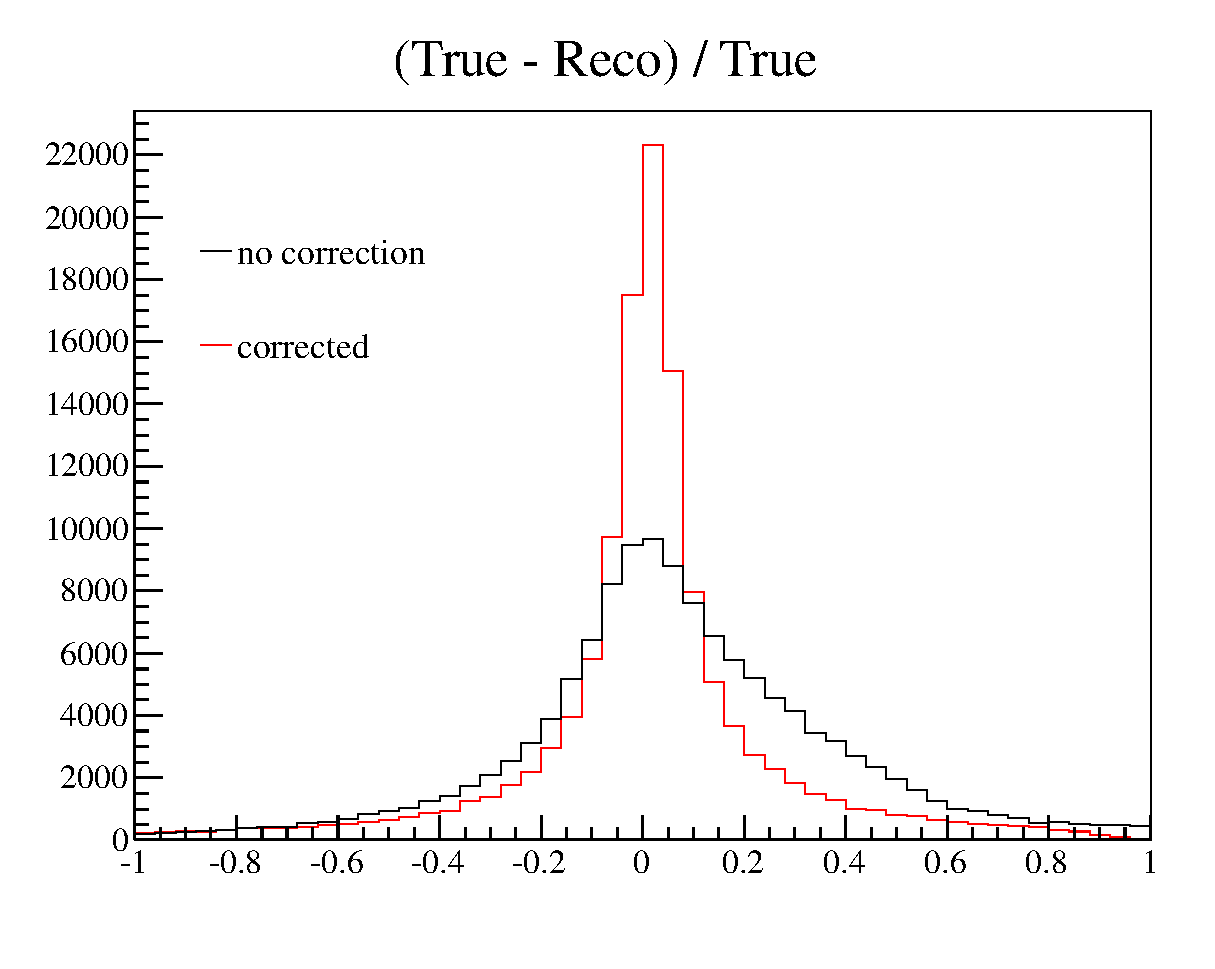
\includegraphics[width=5.5in]{Figures/eCompare.eps}
\caption{Comparison of the global reconstruction \p0d momenta (black) vs manually corrected \p0d momenta (red).  Note that 
the manually corrected momenta are closer to the true momenta and improved compared to global reconstruction.} 
\label{fig:correctedECompare}
\end{figure}

\begin{figure}
\centering
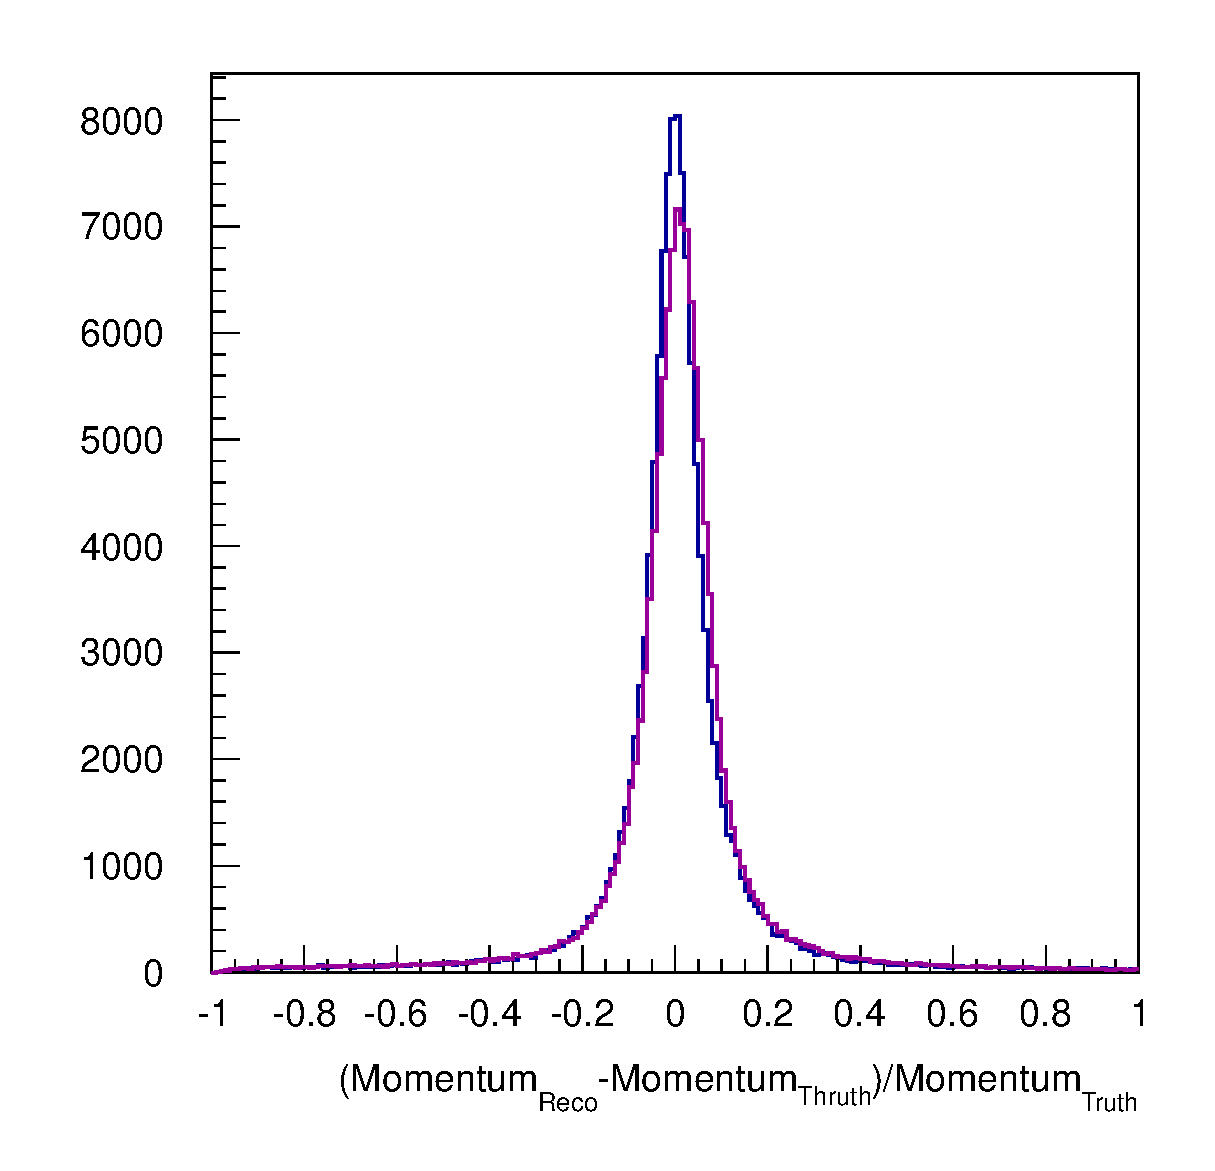
\includegraphics[width=5.5in]{Figures/momentumRecoThruthProd5.eps}
\caption{Comparison of the momenta - Reconstruction (Reco) vs. 
and Trajectory (Truth). The Run 2 (Run 3), Water-in (Water-out), 
period is represented by the Blue (Purpule) curve.}
\label{fig:MomentumComparison}
\end{figure}
